\chapter{Framework Overview}

NOW YOU HAVE SOME THEORY AND PERHAPS A FEW QUANTITATIVE tools at your disposal you are ready to begin creating \textbf{trading systems}. In part three of this book I am going to describe a \textbf{framework} which will provide you with a template for the creation of almost any kind of strategy.

\section*{Chapter overview} \phantomsection \addcontentsline{toc}{section}{Chapter overview}

\begin{chapteroverviewtable}
\chapteroverviewitem{A bad example}{A trading system with some fatal flaws.}
\chapteroverviewitem{Why use a modular framework}{The reasons why a modular framework makes sense for systematic trading strategies.}
\chapteroverviewitem{The elements of the framework}{A brief road map of the various components in the framework.}
\end{chapteroverviewtable}

\medskip

\noindent The following chapters in part three will describe each component in more detail. In the final part of the book I'll show three examples of how this framework can be used, for \textbf{semi-automatic traders}, \textbf{asset allocating investors} and \textbf{staunch systems traders}.

\section*{A bad example} \phantomsection \addcontentsline{toc}{section}{A bad example}

Here's an example of the kind of trading system you find in many books and websites.\footnote{This is a hypothetical example and as far as I know isn't identical to any publicly available system.}

\noindent{\small \setlength{\tabcolsep}{2pt} \renewcommand{\arraystretch}{1.15} 
\begin{tabularx}{\textwidth}{@{} p{0.24\textwidth} Y@{}}
\hline
\textbf{Entry rule} & Buy when the 20 day moving average rises over the 40 day, and vice versa. \\
\hline
\textbf{Exit rule} & Reverse when the entry rule is broken, so if you are long close when the 20 day moving average falls behind the 40 day and go short. \\
\hline
\textbf{Position size} & Never trade more than 10 Eurodollar futures, 1 FTSE contract or £10 per spread bet point. \\
\hline
\textbf{Money management} & Never bet more than 3\% of your capital on each trade. \\
\hline
\textbf{Stop loss} & Set a trailing stop to close once you have lost 3\% of your capital. If you find yourself triggering stops too frequently, then widen them. \\
\hline
\end{tabularx}
}

I am not going to discuss the entry or exit rule.\footnote{The rules aren't too bad, as they are purely systematic and very simple. However they are binary (you're either fully in or out) which isn't ideal, and having only one trading rule variation is also less than perfect.} However the position sizing, money management and stop loss are a mess. 

Firstly why 3\%? Will this generate the right amount of risk? What if I'm particularly conservative, should I still use 3\%? If I don't like a particular trade that much, what should I bet? I typically have 40 positions in my portfolio, so should I be putting 40 lots of 3\% of my portfolio at risk at any one time (meaning 120\% of my total portfolio is at risk)? Does 3\% make sense if I am using a slower trading rule? 

The position sizes above might make sense for someone with an account size of perhaps £50,000 and a certain risk appetite, but what about everyone else? They might be correct when the book was written, but are they still right when we read it five years later? What about an \textbf{instrument} that isn't listed, can we trade it? How? 

Finally, setting a stop loss based solely on your capital and personal pain threshold is incorrect.\footnote{This is recognised by most good traders. Here is Jack Schwager, in Hedge Fund Wizards, interviewing hedge fund manager Colm O'Shea: Jack: "So you don't use stops?" Colm: "No I do. I just set them wide enough. In those early days I wasn't setting stops at levels that made sense on the underlying hypothesis of the trade. I was setting stops based on my pain threshold. When I get out of a trade now it is because I was wrong. ... Prices are inconsistent with my hypothesis. I'm wrong and I need to get out and rethink the situation." (My emphasis.)} Someone with a tiny account who hated losing money would be triggering their very tight stops after a few minutes, whilst a large hedge fund might close a losing position after decades. Stops that would make sense in oil futures would be completely wrong in the relatively quiet USD/CAD FX market. A stop that was correct in the peaceful calm of 2006 would be absurdly tight in the insanity we saw in 2008. 

The solution is to separate out the components of your system: \textbf{trading rules} (including explicit or implicit stop losses), position sizing, and the calculation of your \textbf{volatility target} (the average amount of cash you are willing to risk). You can then design each component independently of the other moving parts. 

Trading rules and stop losses should be based only on expected market price volatility, and should never take your account size into consideration. Calculating a volatility target, how much of your capital to put at risk, is a function of account size and your pain threshold.\footnote{There are other considerations, such as the amount of leverage required versus what is available, and the expected performance of the system. I'll discuss these in more detail in chapter nine, ‘Volatility targeting'.} Positions should then be sized based on how volatile markets are, how confident your price forecasts are, and the amount of capital you wish to gamble. 

Each of these components is part of the modular \textbf{framework} which together form a complete trading system.

\section*{Why a modular framework?} \phantomsection \addcontentsline{toc}{section}{Why a modular framework?}

Remember that I drew an analogy between cars and \textbf{trading systems} in the introduction of this book. \textbf{Trading rules} are the engine of the system. These give you a forecast for instrument prices; whether they are expected to go up or down and by how much.In a car the chassis, drive train and gearbox translate the power the engine is producing into forward movement. Similarly, you will have a position risk management \textbf{framework} wrapped around your trading rules. This translates forecasts into the actual positions you need to hold.

As I said in the introduction the components of a modern car are modular, so they can be individually substituted for alternatives. The trading rules and other components in my framework can also be swapped and changed.

The words module and component could imply that these are complex processes which need thousands of lines of computer code to implement. This is not the case. Every part involves just a few steps of basic arithmetic which require just a calculator or simple spreadsheet.

Let's look in more detail at the advantages of the modular approach.

\subsection*{Flexibility}

The most obvious benefit of a modular design is flexibility. Cars really can be any colour you like, including black. Similarly my framework can be adapted for almost any trading rule, including the discretionary forecasts used by \textbf{semi-automatic traders} and the very simple rule used by \textbf{asset allocating investors}. If you don't like the position sizing component, or any other part of the framework, you can replace it with your own.

\subsection*{Transparent modules}

It's possible to have frameworks that are nicely modular but which contain entirely opaque black boxes. Most PCs are built like this. You can replace the hard disc or graphics card, but you can't easily modify them or make your own, so you are stuck with substituting one mysterious part with another.

In contrast each component in my framework is transparent -- I'll explain how and why it is constructed. This should give you the understanding and confidence to adapt each module, or create your own from scratch.

\subsection*{Individual components with well defined interface}

If you replace the gearbox in your car you need to be sure that the car will still go forward or backwards as required. But if the drive shaft output is reversed on your new gearbox you will end up driving into your front door when you wanted to reverse out of your driveway. To avoid this we need to specify that the shaft on the gearbox must rotate clockwise to make the car go forward, and vice versa.

Similarly if you use a new trading rule then the rest of the modular trading system framework should still work correctly and give you appropriately sized positions. To do this the individual components need to have a well defined interface -- a specification describing how they interact with other parts of the system.

For example in the framework it will be important that a trading rule \textbf{forecast} of say +1.5 has a consistent meaning, no matter what style of trading or instrument you are using.\footnote{It will become clear in later chapters what this consistent meaning is.}

\subsection*{Getting the boring bit right}

The part of the \textbf{trading system} wrapped around the \textbf{trading rules}, the \textbf{framework}, is something that's easily ignored. Creating it is a boring task compared with developing new and exciting trading rules, or making your own discretionary forecasts. But it's incredibly important. By creating a standard framework I've done this dull but vital work for you.

The framework will work correctly for any trading rule that produces forecasts in a consistent way with the right interface. So it won't need to be radically redesigned for any new rules. Also by using the framework \textbf{asset allocating investors} and \textbf{semi-automatic traders} can get much of the benefits of systematic trading without using trading rules to forecast prices.

\subsection*{Examples give you a starting point}

Creating a new \textbf{trading system} from scratch is quite a daunting prospect. In the final part of this book there are three detailed examples showing how the framework can be used to suit \textbf{asset allocating investors}, \textbf{semi-automatic traders} and \textbf{staunch systematic traders}. Together these provide a set of systems you can use as a starting point for developing your own ideas.

\section*{The elements of the framework} \phantomsection \addcontentsline{toc}{section}{The elements of the framework}

Table 15 shows the components you'd have in a small \textbf{trading system} with two \textbf{trading rules}, a total of four trading rule \textbf{variations}, and two \textbf{instruments}. You first create a \textbf{trading subsystem} for each instrument. Each subsystem tries to predict the price of an individual instrument, and calculate the appropriate position required. These subsystems are then combined into a portfolio, which forms the final trading system.

\rawtablecaption{EXAMPLE OF COMPONENTS IN A TRADING SYSTEM}
\begingroup
\centering
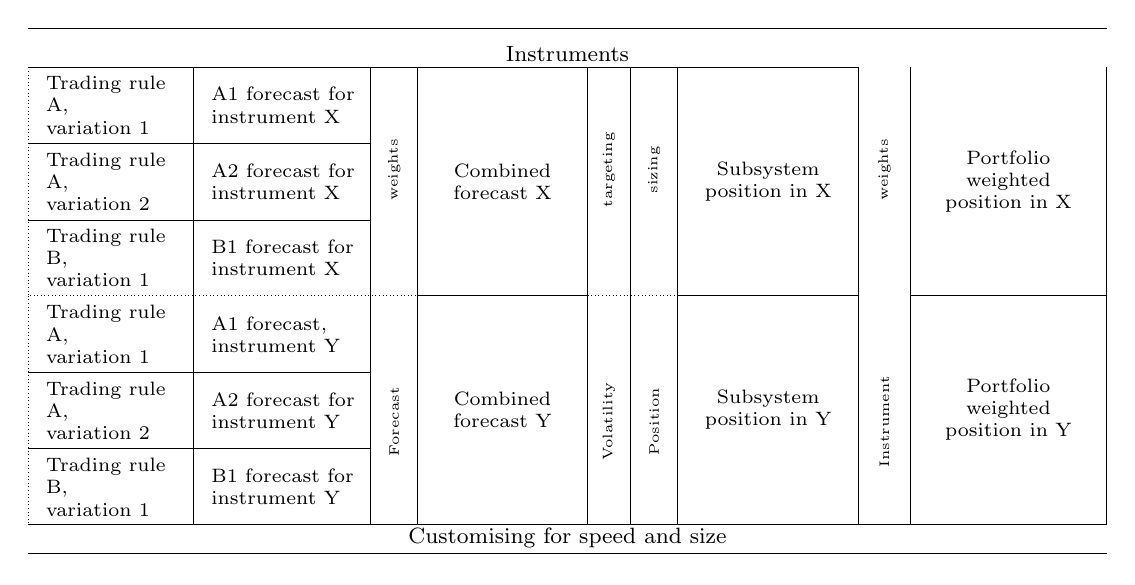
\begin{tikzpicture}[
  x=1cm,
  y=1cm,
  line width=0.3pt,
  font=\booksans\scriptsize,
  boxtext/.style={align=left, inner sep=2.5pt, outer sep=0pt},
  subsystem/.style={densely dotted}
]
\def\xA{0}
\def\xB{2.10}
\def\xC{4.35}
\def\xD{4.95}
\def\xE{7.10}
\def\xF{7.65}
\def\xG{8.25}
\def\xH{10.55}
\def\xI{11.20}
\def\xJ{13.70}

\def\yHeader{6.45}
\def\yTop{5.95}
\def\yOne{4.98}
\def\yTwo{4.01}
\def\yMid{3.05}
\def\yFour{2.08}
\def\yFive{1.11}
\def\yBottom{0.15}
\def\yLabel{-0.02}
\def\yRule{-0.22}

\draw (\xA,\yHeader) -- (\xJ,\yHeader);
\node[font=\booksans\footnotesize] at ({(\xA+\xJ)/2},6.12) {Instruments};

\draw (\xA,\yTop) -- (\xH,\yTop);
\draw (\xB,\yTop) -- (\xB,\yBottom);
\draw (\xC,\yTop) -- (\xC,\yBottom);
\draw (\xD,\yTop) -- (\xD,\yBottom);
\draw (\xE,\yTop) -- (\xE,\yBottom);
\draw (\xF,\yTop) -- (\xF,\yBottom);
\draw (\xG,\yTop) -- (\xG,\yBottom);
\draw (\xH,\yTop) -- (\xH,\yBottom);
\draw (\xI,\yTop) -- (\xI,\yBottom);
\draw (\xJ,\yTop) -- (\xJ,\yBottom);
\draw (\xI,\yMid) -- (\xJ,\yMid);
\draw (\xA,\yBottom) -- (\xJ,\yBottom);

\draw[subsystem] (\xA,\yTop) rectangle (\xH,\yMid);
\draw[subsystem] (\xA,\yMid) rectangle (\xH,\yBottom);

\draw (\xA,\yOne) -- (\xC,\yOne);
\draw (\xA,\yTwo) -- (\xC,\yTwo);
\draw (\xA,\yFour) -- (\xC,\yFour);
\draw (\xA,\yFive) -- (\xC,\yFive);

\draw (\xD,\yMid) -- (\xE,\yMid);
\draw (\xG,\yMid) -- (\xH,\yMid);

\node[boxtext, anchor=west, text width=1.70cm] at (0.14,5.47) {Trading rule A,\\variation 1};
\node[boxtext, anchor=west, text width=1.70cm] at (0.14,4.50) {Trading rule A,\\variation 2};
\node[boxtext, anchor=west, text width=1.72cm] at (0.14,3.53) {Trading rule B,\\variation 1};
\node[boxtext, anchor=west, text width=1.70cm] at (0.14,2.56) {Trading rule A,\\variation 1};
\node[boxtext, anchor=west, text width=1.70cm] at (0.14,1.59) {Trading rule A,\\variation 2};
\node[boxtext, anchor=west, text width=1.72cm] at (0.14,0.62) {Trading rule B,\\variation 1};

\node[boxtext, anchor=west, text width=1.95cm] at (2.24,5.47) {A1 forecast for\\instrument X};
\node[boxtext, anchor=west, text width=1.95cm] at (2.24,4.50) {A2 forecast for\\instrument X};
\node[boxtext, anchor=west, text width=1.95cm] at (2.24,3.53) {B1 forecast for\\instrument X};
\node[boxtext, anchor=west, text width=1.95cm] at (2.24,2.56) {A1 forecast,\\instrument Y};
\node[boxtext, anchor=west, text width=1.95cm] at (2.24,1.59) {A2 forecast for\\instrument Y};
\node[boxtext, anchor=west, text width=1.95cm] at (2.24,0.62) {B1 forecast for\\instrument Y};

\node[rotate=90, font=\booksans\tiny] at ({(\xC+\xD)/2},4.65) {weights};
\node[rotate=90, font=\booksans\tiny] at ({(\xC+\xD)/2},1.45) {Forecast};
\node[boxtext, align=center] at ({(\xD+\xE)/2},{(\yTop+\yMid)/2}) {Combined\\forecast X};
\node[boxtext, align=center] at ({(\xD+\xE)/2},{(\yMid+\yBottom)/2}) {Combined\\forecast Y};
\node[rotate=90, font=\booksans\tiny] at ({(\xE+\xF)/2},4.65) {targeting};
\node[rotate=90, font=\booksans\tiny] at ({(\xE+\xF)/2},1.45) {Volatility};
\node[rotate=90, font=\booksans\tiny] at ({(\xF+\xG)/2},4.65) {sizing};
\node[rotate=90, font=\booksans\tiny] at ({(\xF+\xG)/2},1.45) {Position};
\node[boxtext, align=center] at ({(\xG+\xH)/2},{(\yTop+\yMid)/2}) {Subsystem\\position in X};
\node[boxtext, align=center] at ({(\xG+\xH)/2},{(\yMid+\yBottom)/2}) {Subsystem\\position in Y};
\node[rotate=90, font=\booksans\tiny] at ({(\xH+\xI)/2},4.65) {weights};
\node[rotate=90, font=\booksans\tiny] at ({(\xH+\xI)/2},1.45) {Instrument};
\node[boxtext, align=center] at ({(\xI+\xJ)/2},{(\yTop+\yMid)/2}) {Portfolio\\weighted\\position in X};
\node[boxtext, align=center] at ({(\xI+\xJ)/2},{(\yMid+\yBottom)/2}) {Portfolio\\weighted\\position in Y};

\node[font=\booksans\footnotesize] at ({(\xA+\xJ)/2},\yLabel) {Customising for speed and size};
\draw (\xA,\yRule) -- (\xJ,\yRule);
\end{tikzpicture}\par
\endgroup

\noindent\textit{This trading system has two trading rules A and B; three rule variations A1, A2 and B1; and two instruments X and Y. Dotted lines show trading subsystems for X and Y.}

\subsection*{Instruments to trade}

\textbf{Instruments} are the things you trade and hold positions in. They could be any financial asset including directly held instruments such as equities and bonds, or \textbf{derivatives} like options, futures, contracts for difference and spread bets. You can also trade \textbf{collective funds} such as \textbf{exchange traded funds (ETFs)}, mutual funds, and even hedge funds.

\subsection*{Forecasts}

A \textbf{forecast} is an estimate of how much a particular \textbf{instrument's} price will change, given a particular \textbf{trading rule variation}. For example a simple equities strategy might have three forecasts: two variations on a trend following rule, each looking for different speeds of trend, and a separate equity value trading rule with a single variation. If you are trading two instruments as in table 15 then there will be a total of \(3 \times 2 = 6\) forecasts to make. 

The trading rules which produce forecasts are the engine at the heart of all trading systems used by \textbf{staunch systems traders}. The biggest difference between strategies will be in which rules and variations are used, and which instruments are traded. In comparison the rest of the framework will be fairly similar.

\textbf{Semi-automatic traders} make discretionary forecasts, rather than using systematic rules. \textbf{Asset allocating investors} don't try and predict asset prices and use a single fixed forecast for all instruments.

\subsection*{Combined forecasts}

You need a single forecast of whether an instrument will go up or down in price, and by how much. If you have more than one forecast you will need to combine them into one \textbf{combined forecast} per instrument, using a weighted average. To do this you'll allocate \textbf{forecast weights} to each trading rule variation.

\subsection*{Volatility targeting}

It's important to be precise about how much overall risk you want to take in your trading system. I define this as the typical average daily loss you are willing to expose yourself to. This \textbf{volatility target} is determined using your wealth, tolerance for risk, access to leverage and expected profitability. Initially we'll assume that you're putting all of your capital into a single \textbf{trading subsystem}, for just one instrument.

\subsection*{Scaled positions}

You can now decide how much of the underlying asset to hold based on how risky your instruments are, how confident you are about your \textbf{forecasts}, and your \textbf{volatility target}. The positions you will calculate assume for now that you're just trading one isolated instrument, in a single \textbf{trading subsystem}.

At this point you've effectively got a complete trading system, but for a single instrument. Just as the cells in the human body are each individual living organisms, these trading subsystems are self-contained units, but in the next stage you'll be putting them together.

\subsection*{Portfolios}

To get maximum diversification you'd usually want to trade multiple instruments and put together a portfolio of \textbf{trading subsystems}, each responsible for a single instrument. This requires determining how you are going to allocate capital to the different subsystems in your portfolio, which you will do using \textbf{instrument weights}. After applying this stage you'll end up with \textbf{portfolio weighted positions} in each instrument, which are then used to calculate the trades you need to do.

\subsection*{Speed and Size}

This isn't a separate component in the framework, but a set of principles which apply to the entire system. When designing trading systems it's important to know how expensive they are to trade, and whether you have an unusually large or small amount of capital. Given that information, how should you then tailor your system? I'll address both of these issues in detail in the final chapter of part three.
